% samplepaper.tex: springer.com
% modificato da MM 06/05/2018
%
\documentclass[runningheads]{llncs}
\usepackage[italian]{babel}
\usepackage{graphicx}
\usepackage{subfigure}
% Used for displaying a sample figure. If possible, figure files
% should be included in EPS format.  If you use the hyperref package,
% please uncomment the following line to display URLs in blue roman
% font according to Springer's eBook style:
% \renewcommand\UrlFont{\color{blue}\rmfamily}

\begin{document}
%
\title{Organizzazione e contenuti della relazione di mini-progetto}
%
% \titlerunning{Abbreviated paper title}
% If the paper title is too long for the running head, you can set
% an abbreviated paper title here
%
\author{%
  Filippo Chiandotto\inst{1} \and
  Federico Andreas Dotti\inst{2} \and
  Simone Tosato\inst{3}}
%
\authorrunning{P. Autore et al.}
% First names are abbreviated in the running head.  If there are more
% than two authors, 'et al.' is used.
%
\institute{Corso di laurea magistrale in Scienze Statistiche,
  matricola 1234567 \email{primo.autore@studenti.unipd.it} \and 
  Corso di laurea magistrale in Scienze Statistiche,
  matricola 1234567 \email{primo.autore@studenti.unipd.it} \and 
  Corso di laurea magistrale in Scienze Statistiche,
  matricola 1234567 \email{primo.autore@studenti.unipd.it}}
%
\maketitle        
% typeset the header of the contribution
%
\begin{abstract}
  La relazione si prefigge l’obiettivo di approfondire e affinare metodi di classificazione binaria quali percettroni ed SVM, implementando delle tecniche volte alla riduzione del tempo di esecuzione degli algoritmi e alla loro scalabilità. 
Partendo dalla descrizione del capitolo 12 del libro di testo (Riferimento in bibliografia) e dagli approfondimenti basati sugli articoli è stata proposta una implementazione in Python utilizzando le strutture dati e le operazioni matriciali forniti dal pacchetto numpy (riferimento in bibliografia).   


  \keywords{SVM \and Percettrone \and MapReduce \and Center Distance Ratio Method \and Vettori di supporto }
\end{abstract}

\section{Introduzione}
\label{sec:introduzione}

Il lettore della relazione \`e lo studente medio del corso di laurea
magistrale in Scienze statistiche al quale la relazione deve dare
tutti gli strumenti per comprendere il contenuto.  Ci si metta nei
suoi panni e si scriva tutto ci\`o e solo ci\`e che serve.  Chiedersi
qual \`e il messaggio che lo studente deve ``portarsi a casa'',
esplicitarlo in questo paragrafo e concentrarsi su quello nel resto
della relazione.

L'introduzione della relazione dovr\`a anche illustrare
\begin{itemize}
\item i motivi per i quali il problema affrontato \`e significativo e
\item i metodi utilizzati sono \emph{efficaci} ed \emph{efficienti}.
\end{itemize}
Per significativit\`a s'intende o il mero interesse
teorico-scientifico o l'impatto industriale che avrebbe la soluzione
del problema.  Per efficacia s'intende la capacit\`a di un metodo a
risolvere il problema, mentre l'efficienza \`e relativa al costo
computazionale necessario.

La relazione consiste di quattro paragrafi principali dopo questa
introduzione e prima della bibliografia.  Se il mini-progetto \`e
descrittivo i paragrafi \ref{sec:base-di-partenza} e
\ref{sec:problema-affrontato} devono essere particolarmente accurati
ed estesi.  Per la bibliografia si suggerisce Bib\TeX\ se si scrive con \LaTeX.

\section{Base di partenza}
\label{sec:base-di-partenza}

La base di partenza \`e formata dai metodi documentati nei libri di
testo o negli articoli scientifici.  Variazioni significativi di essi
vanno tra i metodi proposti.  In caso di dubbio si chieda al docente.

Per quanto riguarda gli strumenti \textit{software}, si tenga presente
che l'insegnamento \`e di Informatica e che quindi si preferisce lo
studio, il progetto e l'implementazione di strutture di dati e di
algoritmi ``fatti in casa'' piuttosto che l'utilizzo di ambienti di
sviluppo, come ad esempio Pandas, Julia, R e simili, in cui le
strutture e i programmi sono ``nascosti'' e disponibili come scatole
chiuse.  A lezione sono stati fatti parecchi esempi di cosa s'intende.

Per capire quando dover sviluppare propri algoritmi o strutture di
dati, si provi ad esempio a vedere se i propri metodi sono gi\`a stati
realizzati in qualche ambiente di sviluppo e se hanno tutte le
caratteristiche desiderate, come ad esempio scalabilit\`a e tempi di
esecuzione in ordine polinomiale medio-basso.  Se c'\`e un qualche
``pezzo'' di un metodo di base che non soddisfa almeno un requisito,
come ad esempio la sparsit\`a di una matrice o il tipo di dati
accettati, allora \`e un ``problema'' da affrontare con propri
algoritmi e strutture.

\section{Problema affrontato}
\label{sec:problema-affrontato}

Il problema affrontato dal gruppo deve essere illustrato nel dettaglio
in questo paragrafo.  Si tenga presente che questo insegnamento \`e di
Informatica e quindi sono gli aspetti informatici da mettere in
evidenza.  Durante le lezioni ne sono stati messi in evidenza parecchi
se non addirittura tutti:
\begin{itemize}
\item la dimensione dei dati,
\item il tipo dei dati,
\item il tempo di esecuzione e l'ordine di complessit\`a,
\item lo spazio di memoria di lavoro e quello di disco.
\end{itemize}

\section{Metodi proposti}
\label{sec:metodi-utilizzati}

La metodologia \`e l'insieme coordinato dei metodi che formano la base
di partenza o che sono stati proposti dal gruppo e che quindi sono da
ritenersi un contributo originale.  Non \`e necessario che il gruppo
proponga nuovi metodi, ma se il gruppo ritiene che ci siano, la
relazione deve evidenziarli e dire in cosa si differiscono dalla base
di partenza.

Se il mini-progetto \`e teorico o metodologico allora i risultati
teorici e le metodologie vanno descritti in questo paragrafo.  La
descrizione deve essere rigorosa, non necessariamente matematica.  Si
faccia attenzione alle definizioni.  Se ci sono teoremi gi\`a
riportati in letteratura, \`e sufficiente l'enunciato ed \`e
necessaria la citazione ai lavori scientifici.  I propri teoremi
richiedono una propria dimostrazione che spesso esaurisce il
mini-progetto. 

In ogni caso la descrizione deve essere completa e precisa; poich\'e
la relazione deve essere di 12 pagine al massimo \`e importante che si
scelga con cura cosa scrivere.

\section{Esperimenti}
\label{sec:esperimenti}

Se il mini-progetto \`e sperimentale o empirico gli studi di questo
tipo vanno descritti in questo paragrafo.  Si descrivano le collezioni
di dati in termini di dimensione e tipo ed i risultati dei confronti
tra metodi di base o quelli proposti.  Cruciale \`e la descrizione
accurata degli esperimenti: essa deve permetterne la replicazione.

Il \textit{software}, sia quello a titolo esemplificativo dei concetti
che quello che realizza i propri metodi, va caricato su moodle nella
cartella messa a disposizione pi\`u avanti.  Nella relazione va
scritta la descrizione dell'algoritmo in modo preciso e completo da
permetterne la riproduzione.

\begin{thebibliography}{8}
\bibitem{ref_article1}
Autore, F.: Article title. Journal \textbf{2}(5), 99--110 (2016)

\bibitem{ref_lncs1}
Autore, F., Autore, S.: Title of a proceedings paper. In: Editor,
F., Editor, S. (eds.) CONFERENCE 2016, LNCS, vol. 9999, pp. 1--13.
Springer, Heidelberg (2016). \doi{10.10007/1234567890}

\bibitem{ref_book1}
Autore, F., Autore, S., Autore, T.: Book title. 2nd edn. Publisher,
Location (1999)

\bibitem{ref_proc1}
Autore, A.-B.: Contribution title. In: 9th International Proceedings
on Proceedings, pp. 1--2. Publisher, Location (2010)

\bibitem{ref_url1}
LNCS Homepage, \url{http://www.springer.com/lncs}. Last accessed 4
Oct 2017
\end{thebibliography}

\begin{figure}[h!]
  \subfigure[Primo Autore]{
    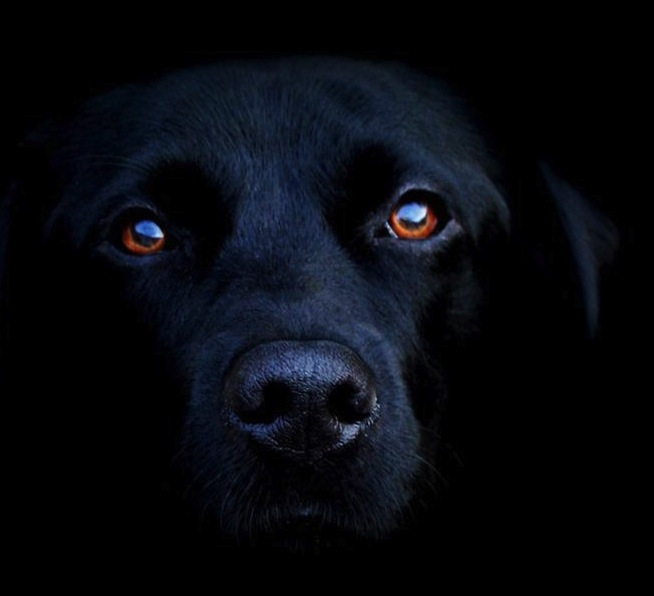
\includegraphics[width=30mm,height=30mm]{dog}}
  \subfigure[Secondo Autore]{
    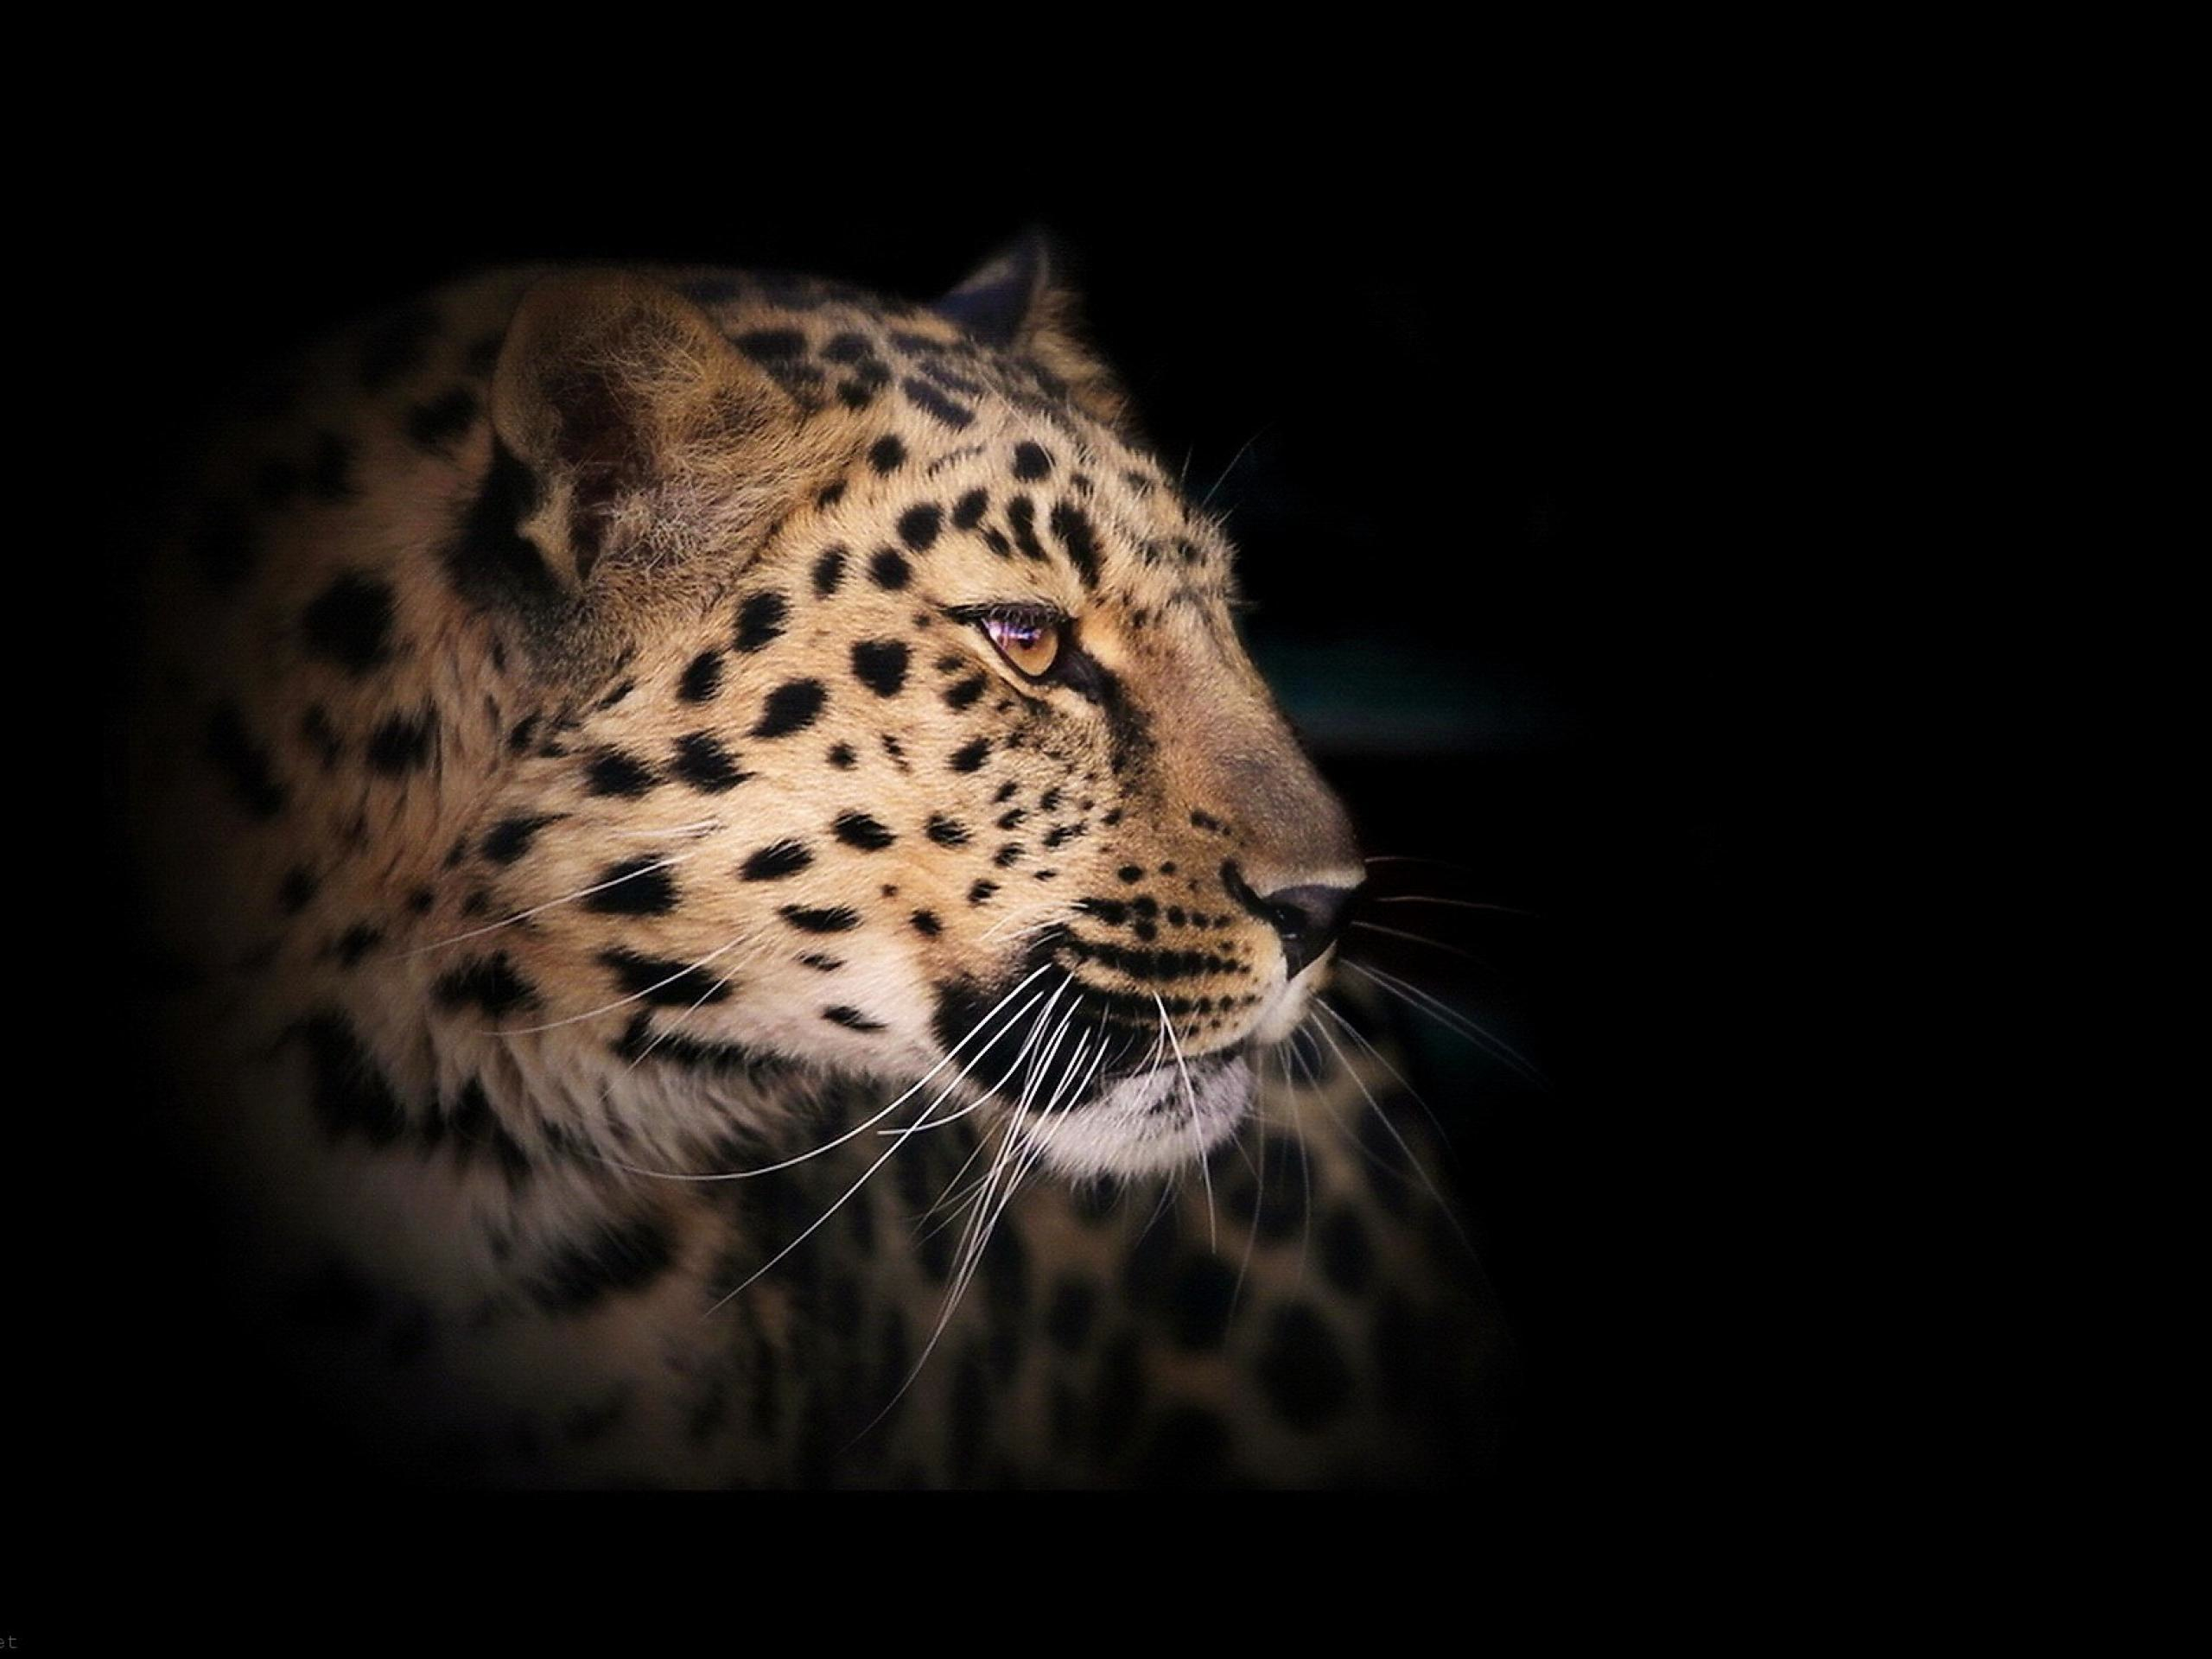
\includegraphics[width=30mm,height=30mm]{tiger}}
  \subfigure[Terzo Autore]{
    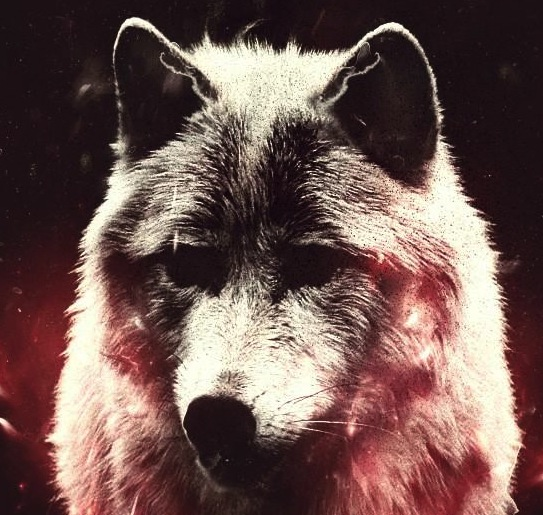
\includegraphics[width=30mm,height=30mm]{wolf}}
\end{figure}

\end{document}
